%%%%%%%%%%%%%%%%%%%%%%%%%%%%%%%%%%%%%%%%%%%%%%%%%%%%%%%%%%%%%%%%%%%%%%
% Based On LaTeX Template: Curriculum Vitae
%
% Source: http://www.howtotex.com/
% Feel free to distribute this template, but please keep the
% referal to HowToTeX.com.
% Date: July 2011
%
%%%%%%%%%%%%%%%%%%%%%%%%%%%%%%%%%%%%%%%%%%%%%%%%%%%%%%%%%%%%%%%%%%%%%%
\documentclass[paper=a4,fontsize=11pt]{scrartcl} % KOMA-article class

\usepackage[english]{babel}
\usepackage[utf8x]{inputenc}
\usepackage[protrusion=true,expansion=true]{microtype}
\usepackage{amsmath,amsfonts,amsthm}     % Math packages
\usepackage{graphicx}                    % Enable pdflatex
\usepackage[svgnames]{xcolor}            % Colors by their 'svgnames'
\usepackage{geometry}
	\textheight=700px                    % Saving trees ;-)
\usepackage{url}
\usepackage{wrapfig}

\frenchspacing              % Better looking spacings after periods
\pagestyle{empty}           % No pagenumbers/headers/footers

%%% Custom sectioning (sectsty package)
%%% ------------------------------------------------------------
\usepackage{sectsty}

\sectionfont{%			            % Change font of \section command
	\usefont{OT1}{phv}{b}{n}%		% bch-b-n: CharterBT-Bold font
	\sectionrule{0pt}{0pt}{-5pt}{3pt}}

%%% Macros
%%% ------------------------------------------------------------
\newlength{\spacebox}
\settowidth{\spacebox}{8888888888}			% Box to align text
\newcommand{\sepspace}{\vspace*{1em}}		% Vertical space macro

\newcommand{\MyName}[1]{ % Name
		\Huge \usefont{OT1}{phv}{b}{n} \hfill #1 %\Huge \fontsize{0}{0}
		\par \normalsize \normalfont}

\newcommand{\MySlogan}[1]{ % Slogan (optional)
		\large \usefont{OT1}{phv}{m}{n}\hfill \textit{#1}
		\par \normalsize \normalfont}

\newcommand{\NewPart}[1]{\section*{\uppercase{#1}}}

\newcommand{\PersonalEntry}[2]{
		\noindent\hangindent=2em\hangafter=0 % Indentation
		\parbox{\spacebox}{        % Box to align text
		\textit{#1}}		       % Entry name (birth, address, etc.)
		\hspace{1.5em} #2 \par}    % Entry value

\newcommand{\SkillsEntry}[2]{      % Same as \PersonalEntry
		\noindent\hangindent=2em\hangafter=0 % Indentation
		\parbox{\spacebox}{        % Box to align text
		\textit{#1}}			   % Entry name (birth, address, etc.)
		\hspace{1.5em} #2 \par}    % Entry value

\newcommand{\EducationEntry}[4]{
		\noindent \textbf{#1} \hfill      % Study
		\colorbox{Black}{%
			\parbox{6em}{%
			\hfill\color{White}#2}} \par  % Duration
		\noindent \textit{#3} \par        % School
		\noindent\hangindent=2em\hangafter=0 \small #4 % Description
		\normalsize \par}

\newcommand{\ExperienceEntry}[4]{ 		% Same as \EducationEntry
		\noindent \textbf{#1} \hfill      % Study
		\colorbox{Black}{%
			\parbox{6em}{%
			\hfill\color{White}#2}} \par  	% Duration
		\noindent \textit{#3} \par        % School
		\noindent\hangindent=2em\hangafter=0 \small #4 % Description
		\normalsize \par}

% \newcommand{\WorkEntry}[4]{				  % Same as \EducationEntry
% 		\noindent \textbf{#1} \hfill      % Jobname
% 		\colorbox{Black}{\color{White}#2} \par  % Duration
% 		\noindent \textit{#3} \par              % Company
% 		\noindent\hangindent=2em\hangafter=0 \small #4 % Description
% 		\normalsize \par}

\newcommand{\CourceEntry}[2]{      % Same as \PersonalEntry
		\noindent\hangindent=2em\hangafter=0 % Indentation
		\parbox{4.2\spacebox}{        % Box to align text
		\textit{#1}}			   % Entry name (birth, address, etc.)
		\hspace{1em} #2 \par}    % Entry value

%%% Begin Document
%%% ------------------------------------------------------------
\begin{document}
% you can upload a photo and include it here...
%\begin{wrapfigure}{l}{0.5\textwidth}
%	\vspace*{-2em}
%		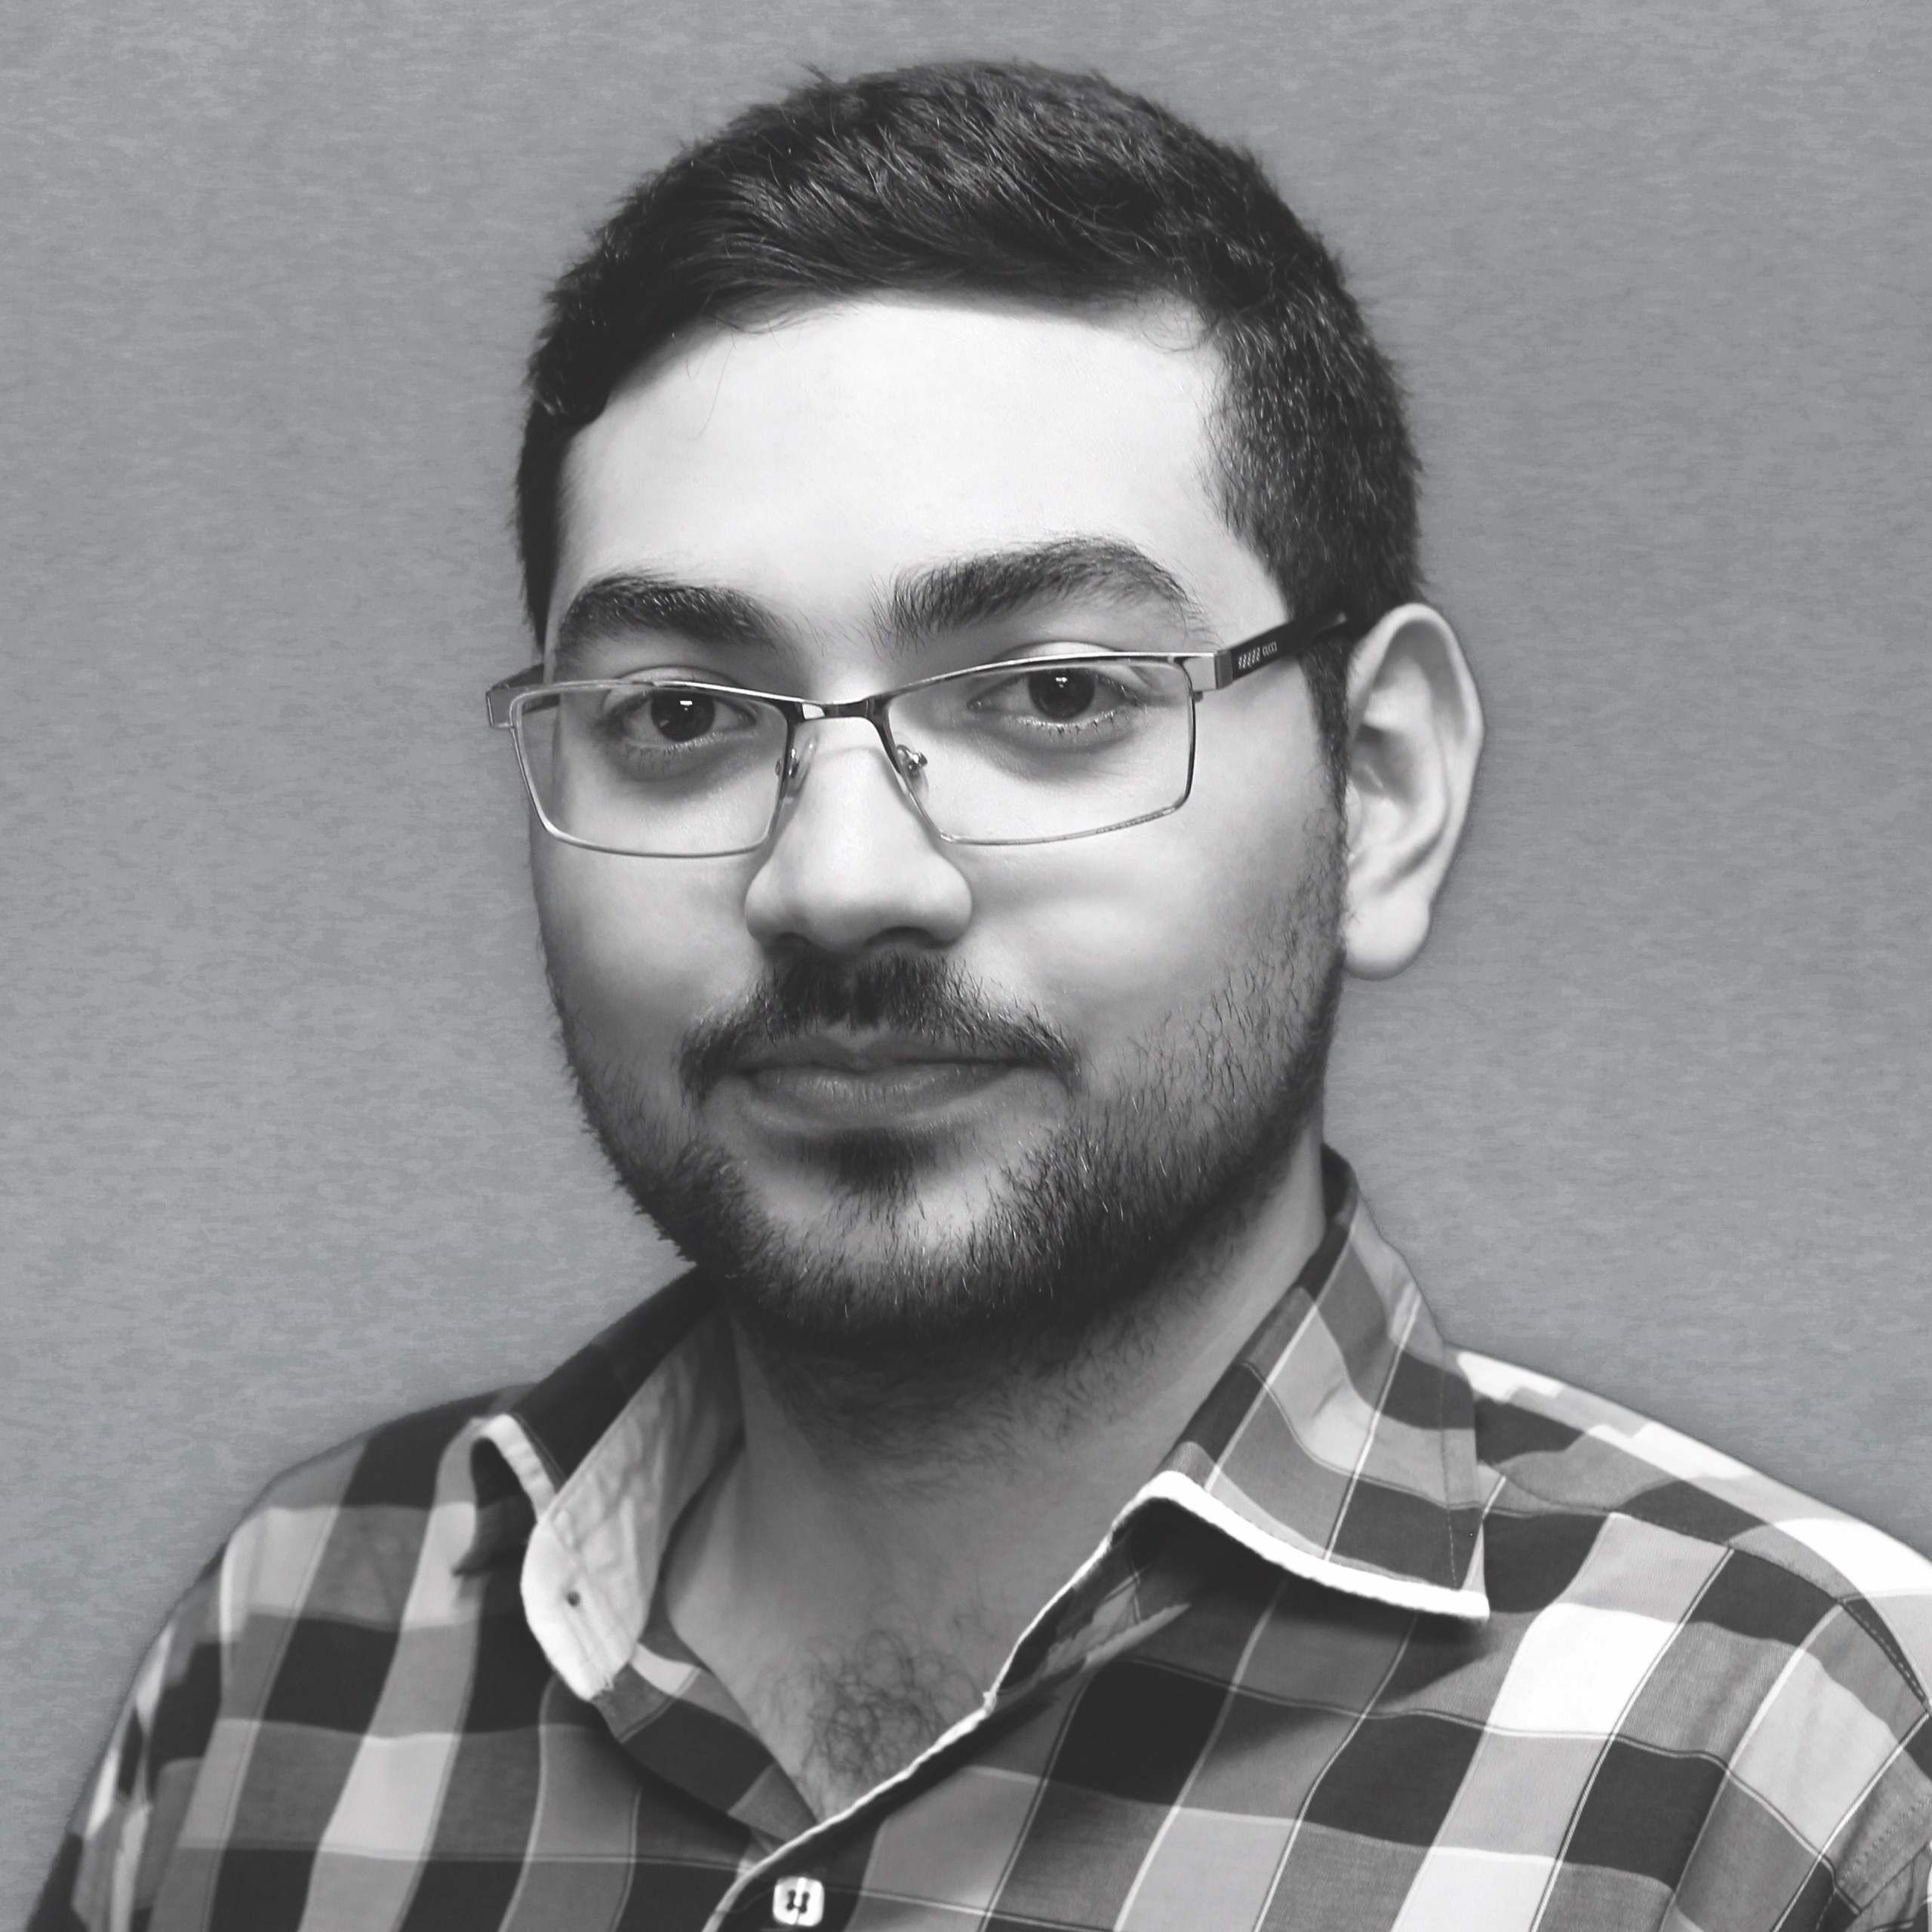
\includegraphics[width=0.15\textwidth]{photo}
%\end{wrapfigure}

\centerline{In the name of Allah, the Most Gracious, the Most Merciful}

\sepspace
\sepspace

\begin{wrapfigure}{l}{0.3\textwidth}
  \vspace*{-3.5em}
  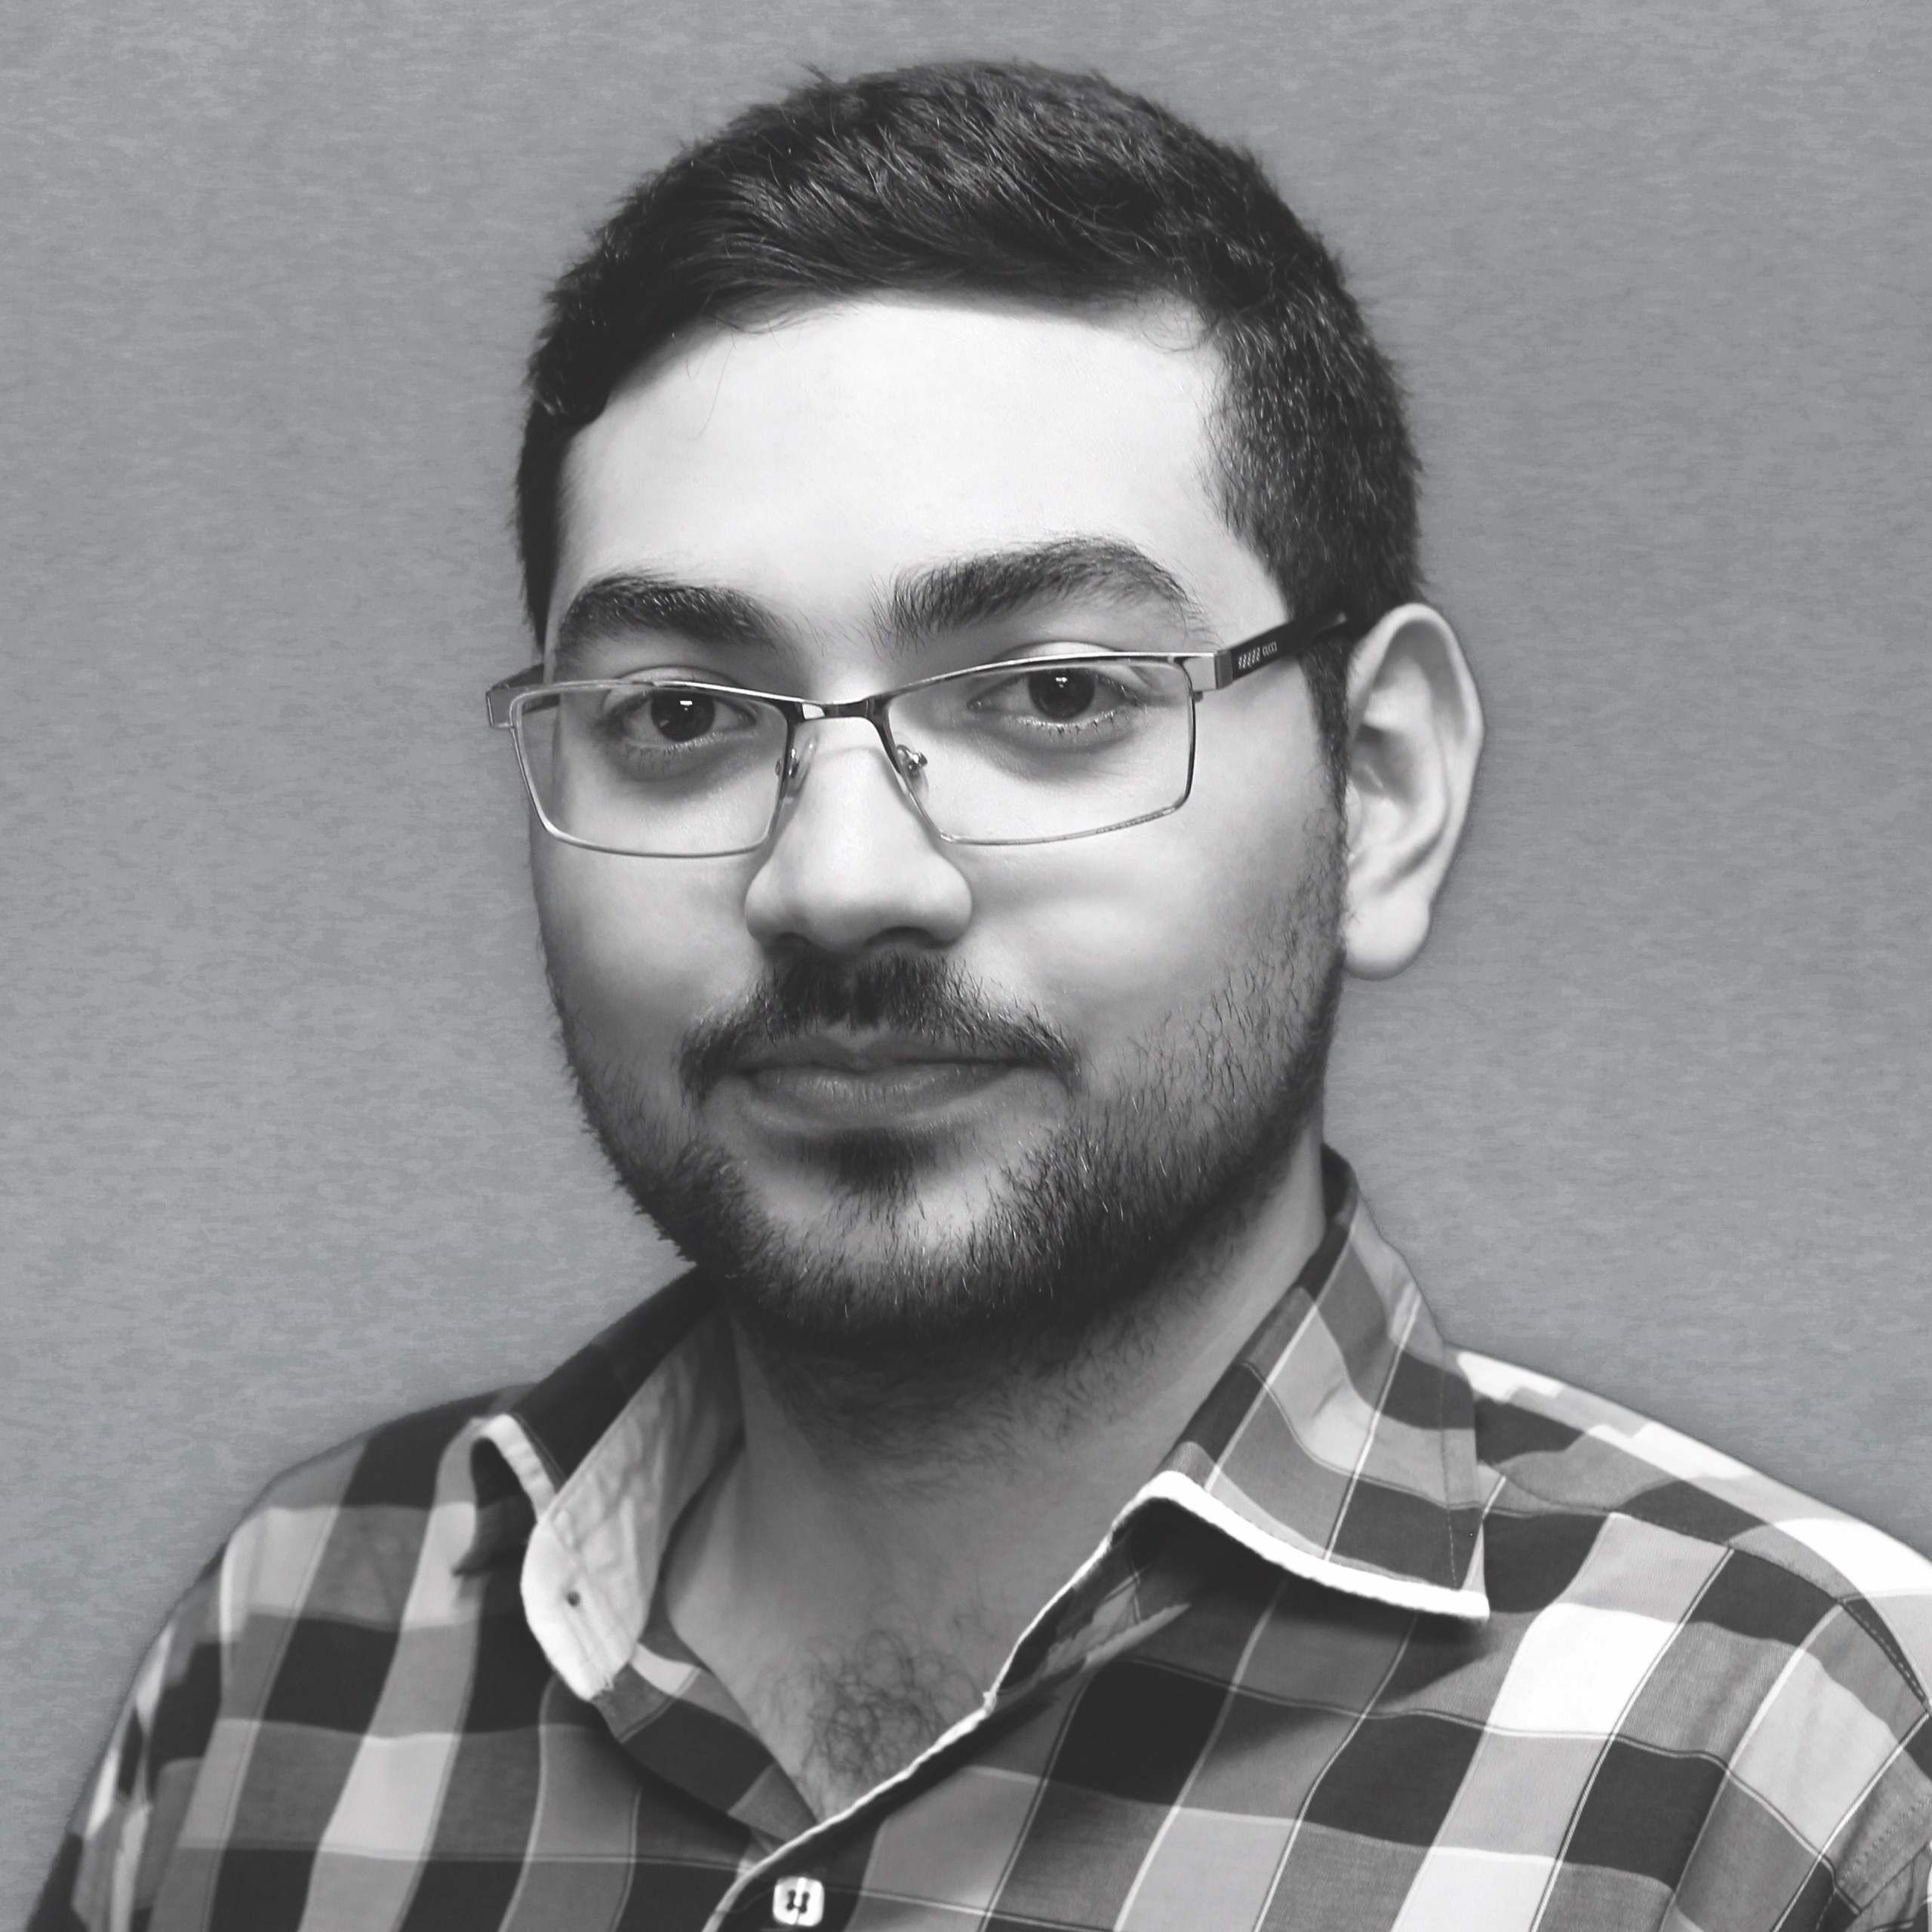
\includegraphics[width=0.2\textwidth]{photo.jpg}
\end{wrapfigure}


\MyName{Mohammad Mohsen}
\MyName{Aseman Manzar}
\MySlogan{97201783}
\MySlogan{}

%%% Personal details
%%% ------------------------------------------------------------
\NewPart{Personal details}{}

\PersonalEntry{Birth}{February 10, 1996}
\PersonalEntry{Phone}{09120728374}
\PersonalEntry{Telegram}{@mohsenasm}
\PersonalEntry{Mail}{\url{m.m.asemanmanzar@gmail.com}}
\PersonalEntry{Linkedin}{\url{https://www.linkedin.com/in/asemanmanzar/}}

%%% Education
%%% ------------------------------------------------------------
\NewPart{Education}{}

\EducationEntry{BSc. Computer Engineering, Software}{2014-2018}{Iran University of Science \& Technology}{\underline{First} Rank, \underline{18.73} GPA}

\sepspace

\EducationEntry{Diploma, Mathematics \& Physics}{2010-2014}{Allameh Tabatabai School}{}

%%% Work experience
%%% ------------------------------------------------------------
\NewPart{Work experience}{}

\ExperienceEntry{iOS/Backend Developer}{2016-present}{Hooshravan}{HooshRavan was born at March 2016 and now the main focus is on "Smart Home Devices". In the market side, The products are known by Hinava brand.}

\sepspace

\ExperienceEntry{Client/Server Developer}{2014-present}{Elmogame Game Studio}{Elmogame studio is a game studio founded by Iran University of Science and Technology students in 2013. Our responsibility is to develop and publish games and despite our team member are students at the same time, so they put some effort on extracurricular academic activities in disparate areas.}

\sepspace

\ExperienceEntry{iOS Developer}{2015-2016}{Hamayeh RnD}{Hamayeh was established in 1995, originally aiming at Automation of Control Systems and in less than 5 years of hard work and experience managed to become the major manufacturer of a wide range of different lighting systems equipment such as Cyclo lights, Flood/Spot Lights, Fresnel Lights, Fluorescent Flood \& Spot Lights, Manual and Motorized Hangers, Digital Dimmers and Lighting Control Systems.}

%%% TA
%%% ------------------------------------------------------------
\NewPart{Teacher Assistant}{}

\ExperienceEntry{Fundamental of Computer Programming}{Fall 2015}{Dr. Adel Torkaman Rahmani}{}
\ExperienceEntry{Advanced Programming}{Spring 2016}{Dr. Adel Torkaman Rahmani}{}
\ExperienceEntry{Principles of Computational Intelligence}{Spring 2018}{Dr. Naser Mozayeni}{}

%%% Courses
%%% ------------------------------------------------------------
\NewPart{Selected Courses}{}

\CourceEntry{Advanced Programming}{20}
\CourceEntry{Discrete Mathematics}{20}
% \CourceEntry{Logic Circuits}{19.75}
\CourceEntry{Data Structures}{20}
\CourceEntry{The Theory of Formal Languages and Automata}{20}
\CourceEntry{System Analysis and Design}{20}
\CourceEntry{Software Engineering}{19}
\CourceEntry{Operating Systems}{19.6}
\CourceEntry{Artificial Intelligence and Expert Systems}{20}
\CourceEntry{Computer Networks}{17.7}
\CourceEntry{Software Testing}{20}
\CourceEntry{Formal Methods in Software Engineering}{20}
\CourceEntry{Object-Oriented Analysis and Design}{19.6}

%%% Projects
%%% ------------------------------------------------------------
\NewPart{Projects}{}

\ExperienceEntry{BSc. Project}{2017-2018}{Supervisor: Dr. Mohammad Abdollahi Azgomi}{Project Title: Mixed Performance and Power Consumption Modeling in Virtual Machine Using Coloured Petri Nets}
\sepspace

\ExperienceEntry{Hinava Smart Home}{2016-present}{iOS/Backend Developer}{Hinava is a smart home system developed in Hooshravan company in Iran. It is one of the first and best manufacturers of smart home systems in the country. The system in Hinava smart home includes three parts; Hardware devices, Hinava cloud service and mobile applications. The devices includes a central panel which acts as a gateway to our system. other devices like sensors and actuators are connected to the central panel and through it they connects to user's app on smartphones or tablets.}
\sepspace

\ExperienceEntry{Kalanshahr Game}{2016-present}{Backend Developer}{Kalanshahr is an online strategy game that each player should manage his/her city by choosing appropriate defensive strategies to avoid rubberily. Each player will build his/her own city and players are usually able to walk around the other players' cities to become aware of their status. Players are also able to watch the inner view of the building in the cities. All resources provided in the game such as police, building, vehicles, etc. are based on the geographical position of cities consist of forest, coastal, desert and urban environment that increases the excitement you could gain from the game.}
\sepspace

% \clearpage

\ExperienceEntry{Footyard Game}{2015-2017}{Unity3D Developer (Physics, Gameplay, AI, etc.)}{Footyard is an online football management game that becomes really more competitive with its devastating online gameplay. Each player will have his/her own team and he/she is responsible for his/her team management. Players are able to injure other players so as long as you have less injured team member then you will win the game against other players. There are the most popular players with their teams from 5 European football leagues besides our exciting domestic football league. It is also possible to find friends and hang out with them.}
\sepspace

\ExperienceEntry{Gametic - A Game Analytics Tool}{2016-2017}{Project Manager, Backend Developer}{Gametic is an analytics tool that specialized for games. Gametic supports many analytics reports in a user-friendly web-based dashboard in two categories of user reports and financial reports. user reports such as daily active users, users retentions and sticky factor. financial report such as ARPU, LTV, Paid Rate.
The major technologies we used was mongodb (sharded cluster), Golang (gin framework) and redis.}
\sepspace

\ExperienceEntry{Farmuler Game}{2015-2016}{Unity3D Developer (Online Gameplay)}{Farmuler is an online multiplayer farm game, that publishes for Android devices. Farmuler has two parts included online multiplayer and offline single player. In offline part, 120 levels are designed and divided into 4 seasons of a year. Players should achieve each level goal at the proper time and they have to demonstrate their skill of time management and resource management to approach the aims. Players will be rewards as they get to the goals sooner.}
\sepspace

%%% Skills
%%% ------------------------------------------------------------
\NewPart{Skills}{}

\SkillsEntry{Language}{\textsc{Persian (mother tongue)}}
\SkillsEntry{}{\textsc{English (limited working proficiency)}}
\sepspace

\SkillsEntry{Programming Language}{\textsc{C\#}, \textsc{Python}, \textsc{Swift}, \textsc{Go}, \textsc{Java}, \textsc{JavaScript}, \textsc{SQL}, \textsc{C/C++}}
\sepspace

\SkillsEntry{Software}{\textsc{Docker}, \textsc{Git}, \textsc{Unity3D}, \textsc{CPN-Tools}}
\sepspace

\SkillsEntry{Industry Knowledge}{\textsc{Backend}, iOS, \textsc{Game Dev.}, \textsc{Web Dev.}, \textsc{Database Design}}
\sepspace

\SkillsEntry{Web Framework}{\textsc{Flask}, \textsc{Django}, \textsc{Gin}}
\sepspace


\end{document}
